% Chapter 6
\chapter{Classification Models and Performance Evaluation}
\label{ch:models}

This chapter compares six classifiers under two imbalance strategies. It first describes the configurations and the training protocol, then reports the performance metrics, the held-out test results, the repeated cross-validation results, the ranking curves, the feature importance analysis, and the pattern matching results. The chapter closes with an interpretation of what the numbers do and do not support.

\section{Classifiers and Configurations}
\label{sec:classifiers}

Six classifiers were chosen to cover different inductive biases: a single tree, a probabilistic baseline, a bagged ensemble, a margin-based method, an instance-based method, and a boosted ensemble. Table~\ref{tab:classifiers} lists them and the reason each was included.

\begin{table}[H]
    \centering
    \caption{Classifiers evaluated in the project.}
    \label{tab:classifiers}
    \begin{tabularx}{\textwidth}{@{}lX@{}}
        \toprule
        \textbf{Classifier} & \textbf{Implementation and role} \\
        \midrule
        Decision Tree & \texttt{DecisionTreeClassifier}. A single axis-aligned tree. It is the most interpretable model in the set and provides a non-ensemble reference point. \\
        Naive Bayes & \texttt{GaussianNB}. A fast probabilistic baseline that assumes conditional independence of the features. \\
        Random Forest & \texttt{RandomForestClassifier}. A bagged ensemble of deep trees. It captures interactions and is robust to irrelevant features. \\
        Support Vector Machine & \texttt{SVC}, wrapped in \texttt{CalibratedClassifierCV}. A margin-based classifier with RBF and linear kernels. It requires scaled inputs. \\
        K-Nearest Neighbours & \texttt{KNeighborsClassifier}. An instance-based classifier that labels a loan by the majority of its nearest neighbours. It also requires scaled inputs. \\
        Gradient Boosting & \texttt{GradientBoostingClassifier}. A sequential ensemble that fits each tree to the residual of the previous ones. \\
        \bottomrule
    \end{tabularx}
\end{table}

Each classifier is evaluated under two imbalance settings. The baseline arm trains on the natural class distribution. The SMOTE arm applies Synthetic Minority Over-sampling Technique inside the pipeline, so the minority class is oversampled to parity within each training fold. The combination gives six models times two settings, or twelve configurations.

The SVM is wrapped in a calibrator because the probability estimates of \texttt{SVC} were deprecated in recent scikit-learn releases. The calibrator is fitted inside the pipeline and does not see the validation fold.

\section{Training Pipeline}
\label{sec:training-pipeline}

The pipeline for each configuration has four steps: optional scaling, optional SMOTE, the classifier, and prediction. Scaling is included for SVM and KNN and omitted for the tree models, which do not need it. The order matters: SMOTE is applied after scaling, so the synthetic points are generated in the same coordinate system as the real ones, and both steps are fitted only on the training portion of each split.

The protocol has three stages.

\begin{enumerate}
    \item \textbf{Single split.} All twelve configurations are trained on the 511-loan training partition with default hyperparameters and scored on the 171-loan test partition.
    \item \textbf{Hyperparameter search.} For each configuration, \texttt{RandomizedSearchCV} samples up to 30 parameter combinations and scores them with F1 on an inner five-fold stratified cross-validation of the training partition. The search never touches the test partition. Naive Bayes has 9 candidates and KNN has 24 because their grids are small.
    \item \textbf{Repeated cross-validation.} The default and tuned versions of all twelve configurations are evaluated with five-fold stratified cross-validation repeated ten times. This produces 50 F1 estimates per configuration and is the table used to select the final model.
\end{enumerate}

The selection metric is mean F1 from the repeated cross-validation. Average precision and ROC-AUC are reported alongside it, but they are not used to re-rank the models after the fact. Fixing the criterion before seeing the results avoids choosing whichever metric happens to favour a preferred model.

\section{Hyperparameter Tuning}
\label{sec:tuning}

Table~\ref{tab:tuning-results} lists the best configuration found for each model and imbalance setting, the number of candidates evaluated, the inner cross-validation F1, and the selected parameters. The search is deliberately modest: 30 candidates per configuration is enough to show whether tuning helps, without turning a 511-row training set into a long optimisation exercise.

\begin{table}[H]
    \centering
    \caption{Hyperparameter search results, ranked by inner cross-validation F1.}
    \label{tab:tuning-results}
    \small
    \begin{tabularx}{\textwidth}{@{}l l r c X@{}}
        \toprule
        \textbf{Model} & \textbf{Arm} & \textbf{Cand.} & \textbf{Inner F1} & \textbf{Best parameters} \\
        \midrule
        Gradient Boosting & Baseline & 30 & 0.582 & \texttt{subsample=0.7; n\_estimators=300; max\_depth=1; learning\_rate=0.05} \\
        Random Forest & SMOTE & 30 & 0.576 & \texttt{n\_estimators=200; min\_samples\_leaf=5; max\_features=sqrt; max\_depth=20} \\
        Gradient Boosting & SMOTE & 30 & 0.538 & \texttt{subsample=0.7; n\_estimators=300; max\_depth=2; learning\_rate=0.05} \\
        SVM & SMOTE & 30 & 0.530 & \texttt{kernel=linear; gamma=0.01; C=100} \\
        Random Forest & Baseline & 30 & 0.519 & \texttt{n\_estimators=200; min\_samples\_leaf=1; max\_features=log2; max\_depth=8} \\
        Decision Tree & SMOTE & 30 & 0.510 & \texttt{min\_samples\_leaf=2; max\_depth=12; criterion=gini; class\_weight=None} \\
        SVM & Baseline & 30 & 0.503 & \texttt{kernel=rbf; gamma=0.01; C=0.1} \\
        Decision Tree & Baseline & 30 & 0.492 & \texttt{min\_samples\_leaf=5; max\_depth=3; criterion=gini; class\_weight=None} \\
        KNN & SMOTE & 24 & 0.385 & \texttt{weights=distance; p=2; n\_neighbors=21} \\
        Naive Bayes & Baseline & 9 & 0.371 & \texttt{var\_smoothing=1e-11} \\
        Naive Bayes & SMOTE & 9 & 0.321 & \texttt{var\_smoothing=1e-11} \\
        KNN & Baseline & 24 & 0.229 & \texttt{weights=uniform; p=2; n\_neighbors=3} \\
        \bottomrule
    \end{tabularx}
\end{table}

The strongest inner-CV result belongs to Gradient Boosting without resampling: 0.582 with a shallow model of 300 stumps, a learning rate of 0.05, and 70\% subsampling. The selected depth of one means each boosting round adds a single split, which keeps the model close to an additive model and limits overfitting on 511 rows.

The tuning curves in Figure~\ref{fig:tuning-curves} show F1 against the key hyperparameter for the two strongest families. The curves are flat over much of the range and then fall sharply. That shape is a warning against reading too much into a small difference between neighbouring settings: the surface is noisy, and the inner CV has only 57 defaults to work with.

\begin{figure}[H]
    \centering
    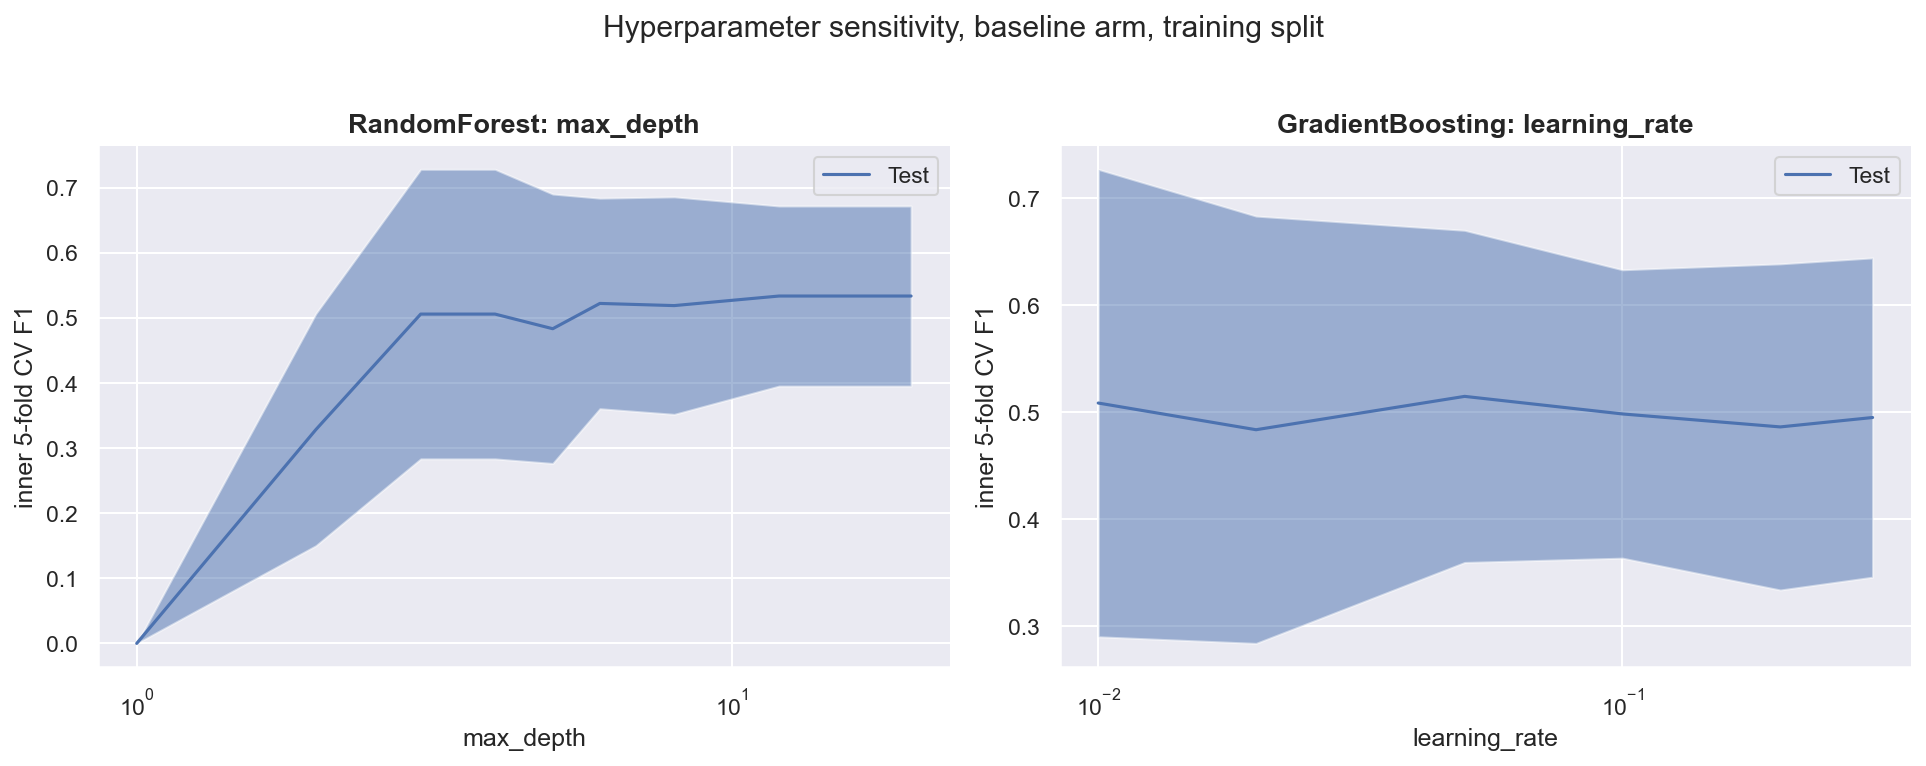
\includegraphics[width=0.95\textwidth]{tuning_curves.png}
    \caption{Hyperparameter sensitivity for the baseline arm on the training split. F1 is flat over a broad region and falls at the extremes.}
    \label{fig:tuning-curves}
\end{figure}

\section{Performance Metrics and Held-Out Test Results}
\label{sec:test-results}

Table~\ref{tab:test-results} reports the single-split results for all twelve configurations with default hyperparameters. The test partition has 171 loans, 19 of which defaulted. A single default therefore moves recall by about 5.3 percentage points, which is the scale against which differences should be read.

\begin{table}[H]
    \centering
    \caption{Held-out test performance with default hyperparameters (171 loans, 19 defaults).}
    \label{tab:test-results}
    \small
    \begin{tabular}{@{}l l r r r r r r@{}}
        \toprule
        \textbf{Model} & \textbf{Arm} & \textbf{Acc.} & \textbf{Prec.} & \textbf{Rec.} & \textbf{F1} & \textbf{AP} & \textbf{AUC} \\
        \midrule
        Random Forest & Baseline & 0.924 & 0.875 & 0.368 & 0.519 & 0.582 & 0.856 \\
        Decision Tree & Baseline & 0.895 & 0.529 & 0.474 & 0.500 & 0.309 & 0.711 \\
        Gradient Boosting & Baseline & 0.912 & 0.700 & 0.368 & 0.483 & 0.583 & 0.816 \\
        SVM & Baseline & 0.918 & 0.857 & 0.316 & 0.462 & 0.551 & 0.771 \\
        Naive Bayes & Baseline & 0.807 & 0.150 & 0.158 & 0.154 & 0.171 & 0.634 \\
        KNN & Baseline & 0.895 & 1.000 & 0.053 & 0.100 & 0.220 & 0.668 \\
        Gradient Boosting & SMOTE & 0.889 & 0.500 & 0.421 & 0.457 & 0.495 & 0.741 \\
        Decision Tree & SMOTE & 0.883 & 0.471 & 0.421 & 0.444 & 0.262 & 0.681 \\
        Random Forest & SMOTE & 0.895 & 0.538 & 0.368 & 0.438 & 0.532 & 0.826 \\
        SVM & SMOTE & 0.854 & 0.375 & 0.474 & 0.419 & 0.385 & 0.726 \\
        KNN & SMOTE & 0.743 & 0.195 & 0.421 & 0.267 & 0.156 & 0.645 \\
        Naive Bayes & SMOTE & 0.591 & 0.108 & 0.368 & 0.167 & 0.155 & 0.563 \\
        \bottomrule
    \end{tabular}
\end{table}

The Random Forest has the highest accuracy (0.924) and precision (0.875), but it catches only 7 of the 19 defaults (recall 0.368). The Decision Tree catches 9 of 19 (recall 0.474) at a lower precision, which gives it the second-best F1. The Gradient Boosting sits between them with an F1 of 0.483 and the highest average precision of the baseline arm (0.583).

The KNN baseline illustrates why precision alone is misleading. It reports a precision of 1.000 because it predicts a single default and gets it right, but its recall is 0.053. A credit team could not use a model that reviews one case and misses eighteen.

SMOTE raises recall for most models but lowers precision by more. The Gradient Boosting arm moves from a recall of 0.368 to 0.421 while precision falls from 0.700 to 0.500. The net F1 is lower. The Naive Bayes SMOTE model is the clearest failure: accuracy falls to 0.591 and precision to 0.108, so the resampling has produced many false alarms without a useful gain in coverage.

Figure~\ref{fig:confusion-matrices} shows the confusion matrices for the twelve configurations. The top row, which contains the baseline models, is dominated by false negatives for the high-precision models. The SMOTE row shifts errors toward false positives. Neither error type is free: a false negative is a missed risky loan, while a false positive is a good customer sent to manual review.

\begin{figure}[H]
    \centering
    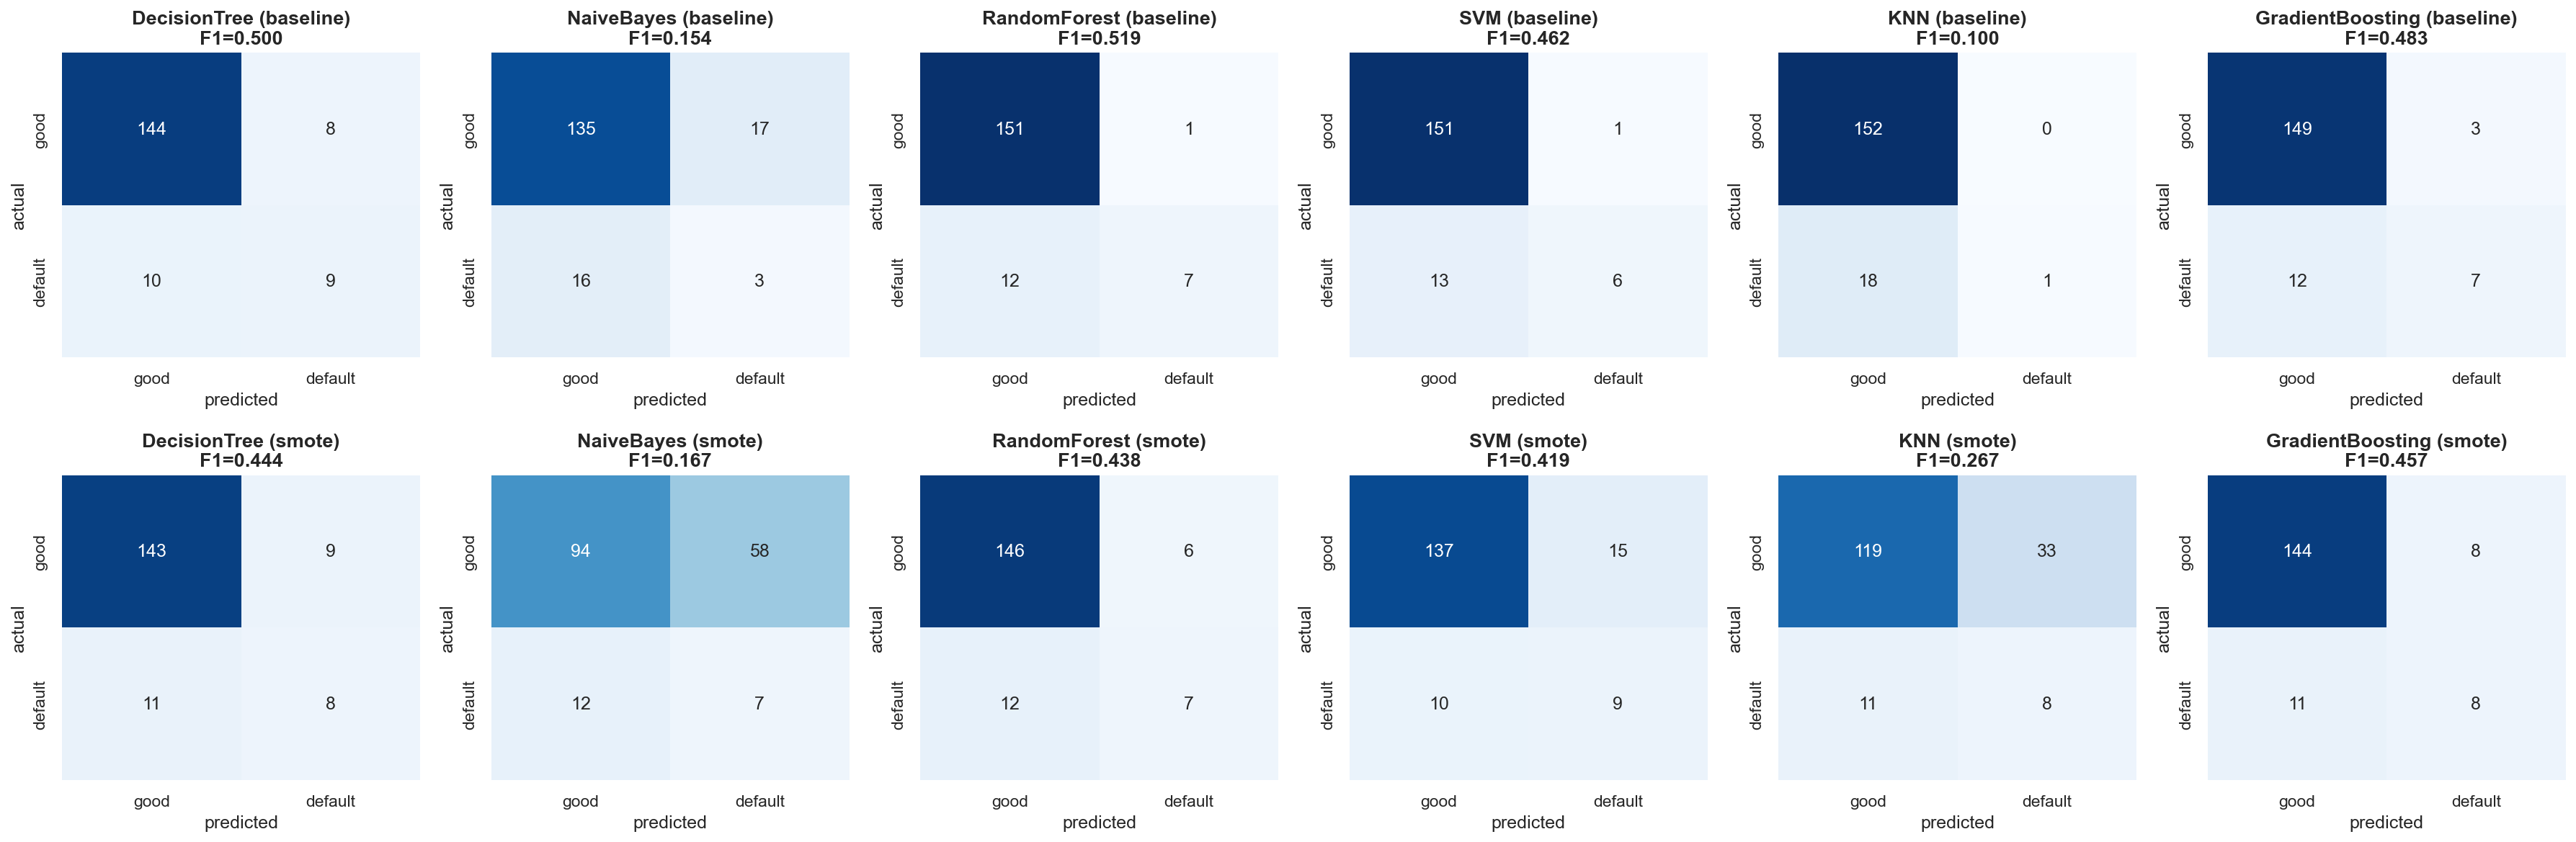
\includegraphics[width=0.95\textwidth]{confusion_matrices.png}
    \caption{Confusion matrices on the held-out test set with default hyperparameters. The two rows show the baseline and SMOTE arms.}
    \label{fig:confusion-matrices}
\end{figure}

\section{Validation Test: Repeated Cross-Validation}
\label{sec:cv-results}

A single test set of 171 loans cannot reliably separate models whose F1 differs by two or three points. Table~\ref{tab:cv-results} therefore reports the mean and standard deviation of F1 over 50 estimates from five-fold cross-validation repeated ten times. The table is ranked by tuned F1, and it includes the default F1 for the same configuration so the effect of tuning is visible.

\begin{table}[H]
    \centering
    \caption{Repeated stratified five-fold cross-validation, ten repeats (50 estimates), ranked by tuned F1. The last two columns describe the tuned configuration.}
    \label{tab:cv-results}
    \small
    \begin{tabular}{@{}l l r r r r@{}}
        \toprule
        \textbf{Model} & \textbf{Arm} & \textbf{F1 default} & \textbf{F1 tuned} & \textbf{AP tuned} & \textbf{AUC tuned} \\
        \midrule
        Gradient Boosting & Baseline & 0.557 & 0.571 $\pm$ 0.120 & 0.654 & 0.864 \\
        Decision Tree & Baseline & 0.491 & 0.557 $\pm$ 0.126 & 0.507 & 0.748 \\
        Random Forest & Baseline & 0.557 & 0.556 $\pm$ 0.112 & 0.661 & 0.877 \\
        Random Forest & SMOTE & 0.537 & 0.542 $\pm$ 0.103 & 0.638 & 0.872 \\
        Gradient Boosting & SMOTE & 0.542 & 0.536 $\pm$ 0.101 & 0.641 & 0.851 \\
        SVM & Baseline & 0.421 & 0.498 $\pm$ 0.128 & 0.603 & 0.842 \\
        Decision Tree & SMOTE & 0.452 & 0.464 $\pm$ 0.104 & 0.307 & 0.741 \\
        SVM & SMOTE & 0.436 & 0.463 $\pm$ 0.084 & 0.608 & 0.848 \\
        KNN & SMOTE & 0.336 & 0.367 $\pm$ 0.065 & 0.367 & 0.768 \\
        Naive Bayes & Baseline & 0.325 & 0.325 $\pm$ 0.132 & 0.356 & 0.769 \\
        Naive Bayes & SMOTE & 0.318 & 0.318 $\pm$ 0.055 & 0.338 & 0.729 \\
        KNN & Baseline & 0.198 & 0.223 $\pm$ 0.129 & 0.249 & 0.628 \\
        \bottomrule
    \end{tabular}
\end{table}

Gradient Boosting with the baseline arm has the highest mean tuned F1 at 0.571. Random Forest is second at 0.556 and has the best average precision (0.661) and ROC-AUC (0.877). The F1 gap between them is 0.015, while the fold-to-fold standard deviation is about 0.11. The two models are effectively tied on F1, and the Random Forest ranks positives better. The selection rule nevertheless points to Gradient Boosting because F1 was fixed as the criterion before the comparison. The report keeps Random Forest as a credible alternative rather than pretending the choice is unambiguous.

The Decision Tree is the surprise of the table. Tuning raises its F1 from 0.491 to 0.557, a gain of 0.066, and places it third. Its average precision is only 0.507, however. The tree has learned a decision boundary that captures more defaults at the cost of a less reliable ranking. This is the clearest example of why F1 and AP should be read together: they answer different questions.

The tuning gains are uneven. The SVM improves by 0.077 and the Decision Tree by 0.066, while the Random Forest does not improve at all ($-0.001$) and Naive Bayes is unchanged. The models with strong default settings had less room to gain, and the search may simply have confirmed that their defaults were already appropriate for this sample size.

SMOTE helps only KNN at the tuned comparison (0.223 to 0.367). For the other five models, the tuned baseline arm is at least as good as the tuned SMOTE arm. The result is consistent with the test table and with the small absolute number of defaults: synthetic minority points can smooth a boundary that is already hard to estimate, and the extra recall often arrives with a larger loss in precision. The project therefore does not recommend SMOTE as a default for this dataset.

Figure~\ref{fig:cv-selection} shows the tuning gain for each configuration, with the selected model marked. The visual makes the two large gains (SVM and Decision Tree) and the flat response of the already-strong models easy to see.

\begin{figure}[H]
    \centering
    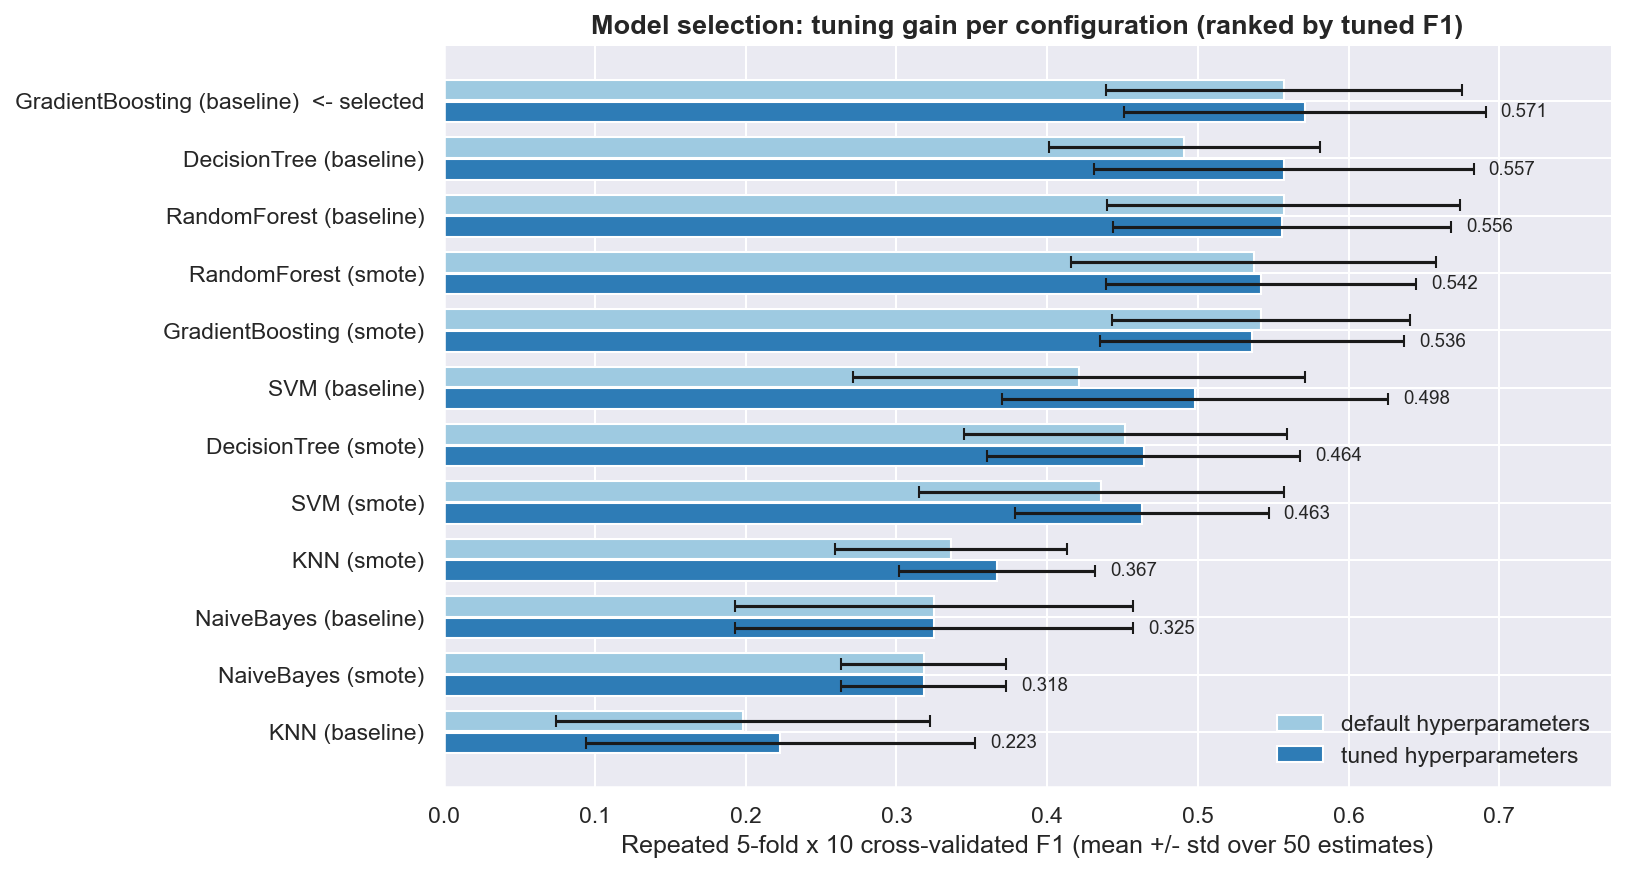
\includegraphics[width=0.9\textwidth]{cv_selection.png}
    \caption{Tuning gain per configuration under repeated cross-validation. The selected Gradient Boosting baseline is marked.}
    \label{fig:cv-selection}
\end{figure}

\section{Ranking Curves}
\label{sec:ranking-curves}

Figures~\ref{fig:roc-curves} and~\ref{fig:pr-curves} show the ROC and precision-recall curves for the default configurations. The ROC curves of Random Forest, Gradient Boosting, and SVM sit well above the diagonal, with AUC values in the 0.77 to 0.86 range on the test set. The precision-recall curves are more sobering. At an 11.14\% prevalence, the no-skill average precision is 0.111, and the best default model reaches about 0.58. That is a real improvement, but it is far from a clean separation.

\begin{figure}[H]
    \centering
    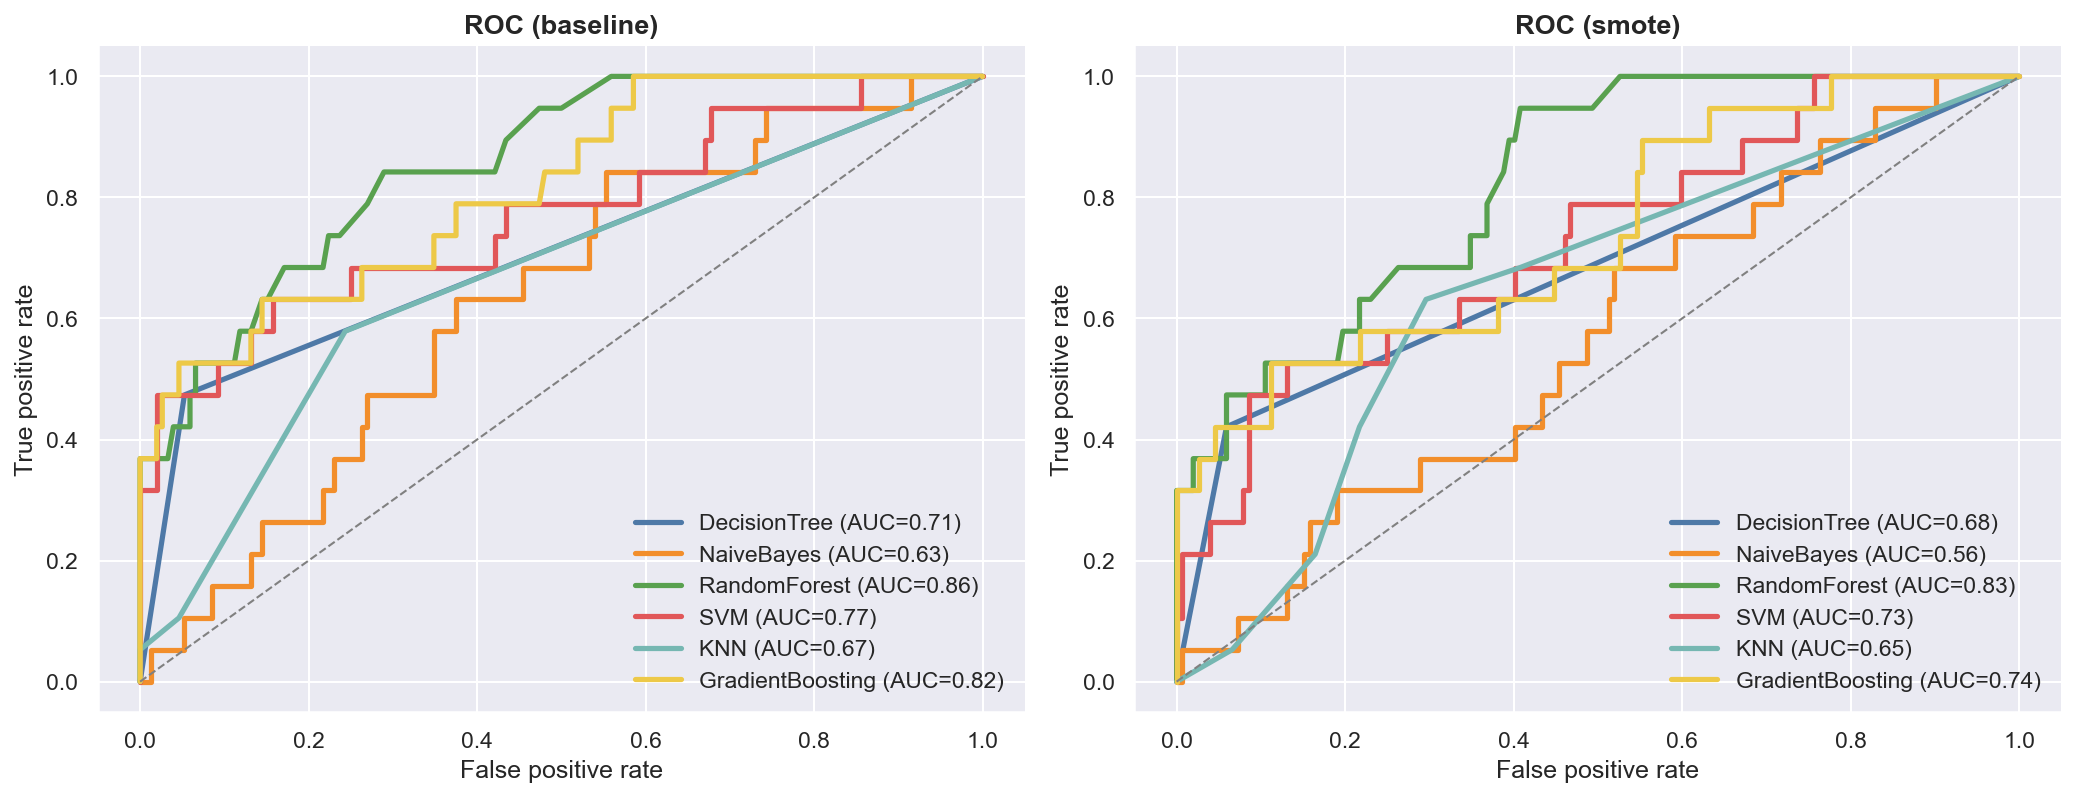
\includegraphics[width=0.95\textwidth]{roc_curves.png}
    \caption{ROC curves by imbalance arm on the held-out test set, default hyperparameters.}
    \label{fig:roc-curves}
\end{figure}

\begin{figure}[H]
    \centering
    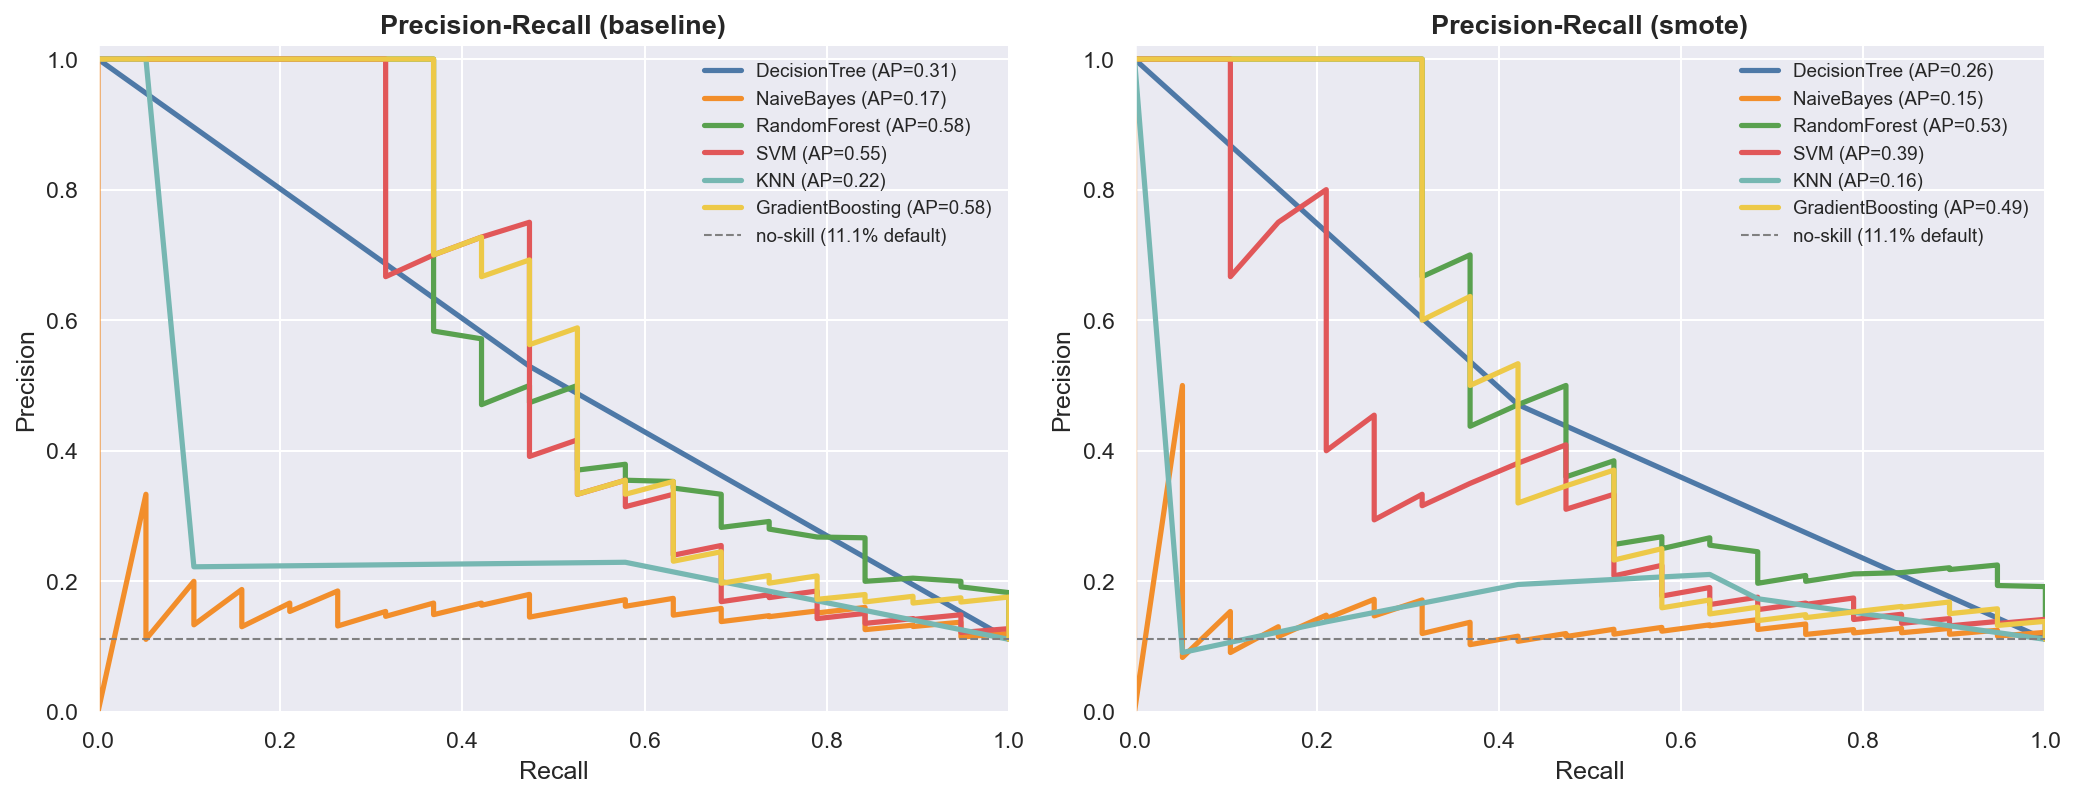
\includegraphics[width=0.95\textwidth]{pr_curves.png}
    \caption{Precision-recall curves with average precision on the held-out test set, default hyperparameters. The dashed baseline is the 11.14\% default rate.}
    \label{fig:pr-curves}
\end{figure}

The ROC view can flatter a model on imbalanced data because a large number of true negatives keeps the false-positive rate low even when many defaults are missed. The precision-recall view makes the cost visible: to reach a recall of 0.5, a model must accept a precision well below its peak. The operating threshold is therefore a business decision, not a property of the classifier.

\section{Feature Importance}
\label{sec:feature-importance}

Figure~\ref{fig:rf-importance} shows impurity-based importance from the tuned Random Forest. The Random Forest is used for this view because tree ensembles expose a direct importance score and the tuned forest was one of the two strongest models. The scores are not causal effects; they describe how much a feature contributed to reducing impurity across the forest.

\begin{figure}[H]
    \centering
    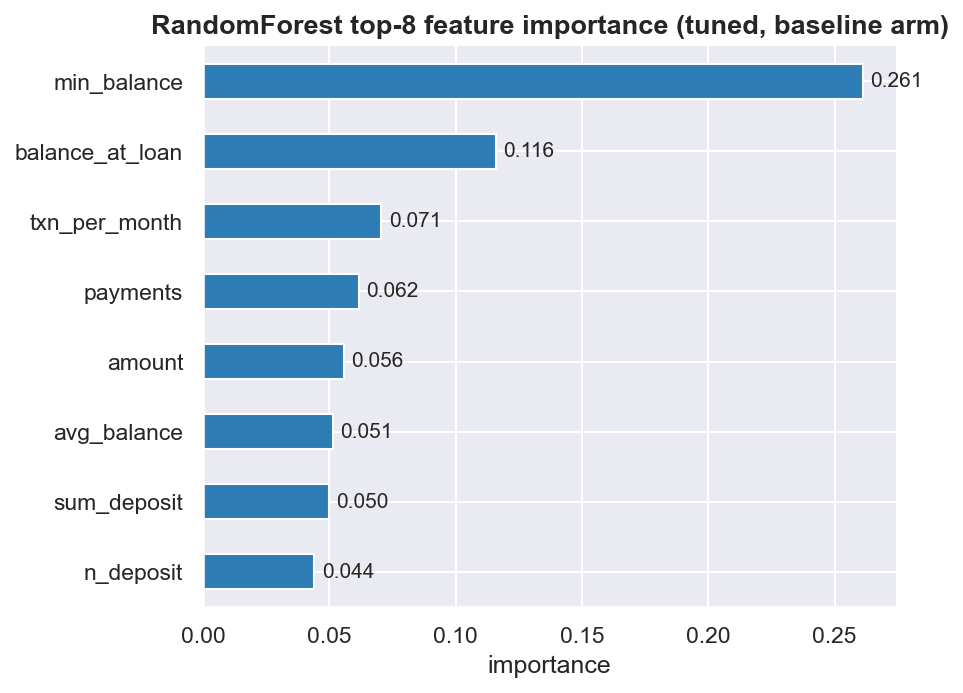
\includegraphics[width=0.62\textwidth]{rf_importance.png}
    \caption{Feature importance from the tuned Random Forest. Balance features dominate; demographic features contribute little.}
    \label{fig:rf-importance}
\end{figure}

\texttt{min\_balance} is the single most important feature at 0.261, followed by \texttt{balance\_at\_loan} at 0.116. The two balance features together account for more than a third of the total importance. Transaction frequency (0.071), monthly payment (0.062), loan amount (0.056), and average balance (0.051) form a second tier. Age (0.025) and gender (0.005) are near the bottom.

Two cautions apply. First, impurity importance is biased toward features with many distinct values, and all the money and count features are continuous. Second, correlated features share credit: when \texttt{sum\_deposit} and \texttt{sum\_withdrawal} carry almost the same information, the forest may split on either one, and their individual scores can change between runs. The grouped conclusion is safer than any single rank: balance history and loan burden carry the signal, while demographics do not.

\section{Pattern Matching with Apriori and FP-Growth}
\label{sec:pattern-mining}

The pattern mining step looks for simple co-occurrences between pre-loan behaviours and default. It uses Apriori and FP-Growth on one basket per account, built from the first loan on the account and transactions dated before that loan. An item records whether the account ever showed a behaviour in that window. The minimum support is 0.03, the maximum itemset length is three, the minimum confidence is 0.10, and rules are kept only if the lift is above 1.0 and the consequent is default. Redundant rules are pruned when a more general rule is at least as strong.

Both algorithms return the same 41 itemsets and the same two default-oriented rules, which is a useful consistency check. Table~\ref{tab:pattern-rules} reports the rules.

\begin{table}[H]
    \centering
    \caption{Default-oriented association rules after redundancy pruning. Support is the share of the 682 accounts; coverage is the share of the 76 defaults.}
    \label{tab:pattern-rules}
    \begin{tabular}{@{}l r r r r@{}}
        \toprule
        \textbf{Antecedent} & \textbf{Antecedent support} & \textbf{Confidence} & \textbf{Lift} & \textbf{Default coverage} \\
        \midrule
        \texttt{negative\_balance} & 3.96\% (27/682) & 100.0\% & 8.97 & 35.5\% (27/76) \\
        \texttt{type\_VYBER} & 54.11\% (369/682) & 13.0\% & 1.17 & 63.2\% (48/76) \\
        \bottomrule
    \end{tabular}
\end{table}

The first rule is striking: all 27 accounts that ever had a negative running balance before the first loan defaulted. The lift of 8.97 and the confidence of 1.000 make it the strongest pattern in the data. It is also a small group, so the confidence interval around 100\% is wide, and the rule is univariate: it does not control for loan size, history length, or the other behaviours. It should be read as a signal worth investigating, not as a lending policy.

The second rule is weak. Accounts that used cash withdrawals (VYBER) default at 13.0\%, barely above the 11.14\% base rate, for a lift of 1.17. The rule covers 48 defaults because cash withdrawals are common (54.11\% of accounts), not because they are dangerous. It is reported for completeness and is not actionable on its own.

The difference between the two rules is a useful summary of the whole analysis. A rare, extreme behaviour (a negative balance) is highly predictive but covers a minority of defaults. A common behaviour (cash withdrawal) covers many defaults but barely improves on the base rate. A usable system needs both: a high-precision rule for a small group, and a model that ranks the rest of the portfolio.

\section{Discussion}
\label{sec:model-discussion}

The results support four conclusions.

\begin{itemize}
    \item \textbf{The top models are close.} Gradient Boosting and Random Forest are separated by 0.015 F1 under repeated cross-validation, with fold-to-fold standard deviations around 0.11. The choice of Gradient Boosting follows the pre-specified F1 criterion, but Random Forest has better average precision and ROC-AUC and is a defensible alternative.
    \item \textbf{SMOTE is not a default fix.} It improves KNN and raises recall for several models, but it lowers F1 for five of six tuned configurations. With 76 defaults, synthetic samples do not add enough new information to justify the precision loss.
    \item \textbf{Tuning helps some models a lot and others not at all.} The SVM gains 0.077 F1 and the Decision Tree 0.066, while the Random Forest and Naive Bayes are flat. Hyperparameter search is most useful when the default model is poorly matched to the data scale or the tree depth.
    \item \textbf{Ranking metrics change the story.} The Decision Tree reaches a respectable F1 after tuning but has a much lower average precision than the forest. A credit team that reviews the highest-risk cases should care about the ranking, not only about the thresholded F1.
\end{itemize}

The limitations are equally important. The test set contains 19 defaults, so a single split has wide uncertainty. The cross-validation reuses the same folds for tuning and reporting, which makes the tuned means mildly optimistic; a nested cross-validation would give a cleaner estimate of the tuning procedure. The data is a 1990s Czech retail portfolio and does not represent current borrowers. The features describe account behaviour, not income, employment, or credit bureau history, so the model cannot see the most common reasons for default. Finally, the predicted scores are ranks, not calibrated probabilities. A threshold of 0.5 has no special meaning without calibration, and the review queue uses the ranking rather than a fixed probability cutoff.

\section{Interactive Review Console}
\label{sec:streamlit}

The results are exposed through a Streamlit application, started with \texttt{streamlit run app.py}. The application does not retrain models; it reads the CSV artifacts written by the notebooks. It has four pages.

\begin{enumerate}
    \item \textbf{Model comparison.} A table of the twelve configurations with the held-out metrics, plus the ROC and precision-recall curves. This page answers the question ``how do the models compare?'' at a glance.
    \item \textbf{Why the best model.} The tuning result, the selected parameters, and the feature importance chart. This page explains what the selected model relies on and where its limits are.
    \item \textbf{Review queue.} A ranked list of loans by out-of-fold default probability, with a threshold slider. The probabilities come from five-fold out-of-fold predictions over all 682 loans, not from resubstitution on the training data. The page states that the cutoff prioritises manual review; it is not an approval decision.
    \item \textbf{FP-Growth and patterns.} The mined itemsets, the two default rules, and their support, confidence, and lift. This page connects the model results to the simpler rule-based view.
\end{enumerate}

The separation between training and serving matters. A dashboard that retrained on every page load would produce numbers that drift from the report and would make the review queue depend on the current random state. By freezing the artifacts, the console shows exactly the results discussed in this chapter.

The next chapter draws the results together, states the recommendation, and sets out the limitations and the work that would be needed before deployment.
